

We note there are problems one can formulate where the observed density corresponds directly to a normalized likelihood function familiar to Bayesian statisticians, as we demonstrate below.
One difference between $\updated$ and $\posterior$ is the use of normalizing constant $C$ in $\posterior$ not present in $\updated$, as explained by Corollary~\ref{cor:int} above.
To illustrate the differences in the two densities, we explore the impact of this difference in the example below, taken from \cite{BJW18}.

%%%%%



Suppose $\pspace = [-1,1]\subset\RR$ and $Q(\param)=\param^5$ so that $\dspace = [-1,1]$.
For the observation-consistent framework, we assume $\initial\sim \mathcal{U}([-1,1])$ and $\observed\sim N(0.25,0.1^2)$.
The push-forward of initial PDF, the observed PDF, and the updated PDF are shown in Fig.~\ref{fig:bayes-comparison}.

For the Bayesian inverse problem, we assume $d\in \dspace$ with $d=Q(\paramref)+\xi$ where $\xi\sim N(0,0.1^2)$.
%In particular, we assume that $d=0.25$ and follow the process of \cite{Stuart_Bayesian} to form the data-likelihood function so that it matches the observed density.
We then construct $\pi_{\text{post}}(\param \, |\, d)$ for this example assuming a uniform prior (to match the initial density) with an assumed observed value of $d=0.25$ so that the data-likelihood function matches the observed density.
The posterior and its push-forward are also shown in Fig.~\ref{fig:bayes-comparison}.

While the updated and posterior densities in Fig.~\ref{fig:bayes-comparison} share certain similarities (e.g., they are uni-modal with similar locations of the mode), they are otherwise visibly distinct.
The differences between these densities is made more evident by examining their push-forwards.
The push-forward of the updated density agrees well with the observed density, which is to be expected.
However, the push-forward of the posterior is bi-modal and does not match the observed density, which we recall is identical to the data-likelihood function in this case.
%with peaks that appear to align fairly well with the two distinct peaks of the predicted density and observed density.
%Recall that the observed density and data-likelihood are, in this case, identical.
%Moreover, with the setup described above, the predicted density can also be interpreted as the push-forward of the prior density.
%This demonstrates the regularizing impact of the prior on the posterior and how i.

%
%Hierarchical Bayesian methods \cite{} extend this typical framework to problems where aleatoric uncertainties are present, but are still fundamentally developed from a  point estimation perspective.
%Specifically, prior distributions are specified from a parametric family of distributions, such as Gaussian distributions, and the hyper-parameters used to define that family of distributions, such as the means and variances, become a focal point of estimation by the methodology.


\begin{figure}[htbp]
\centering
   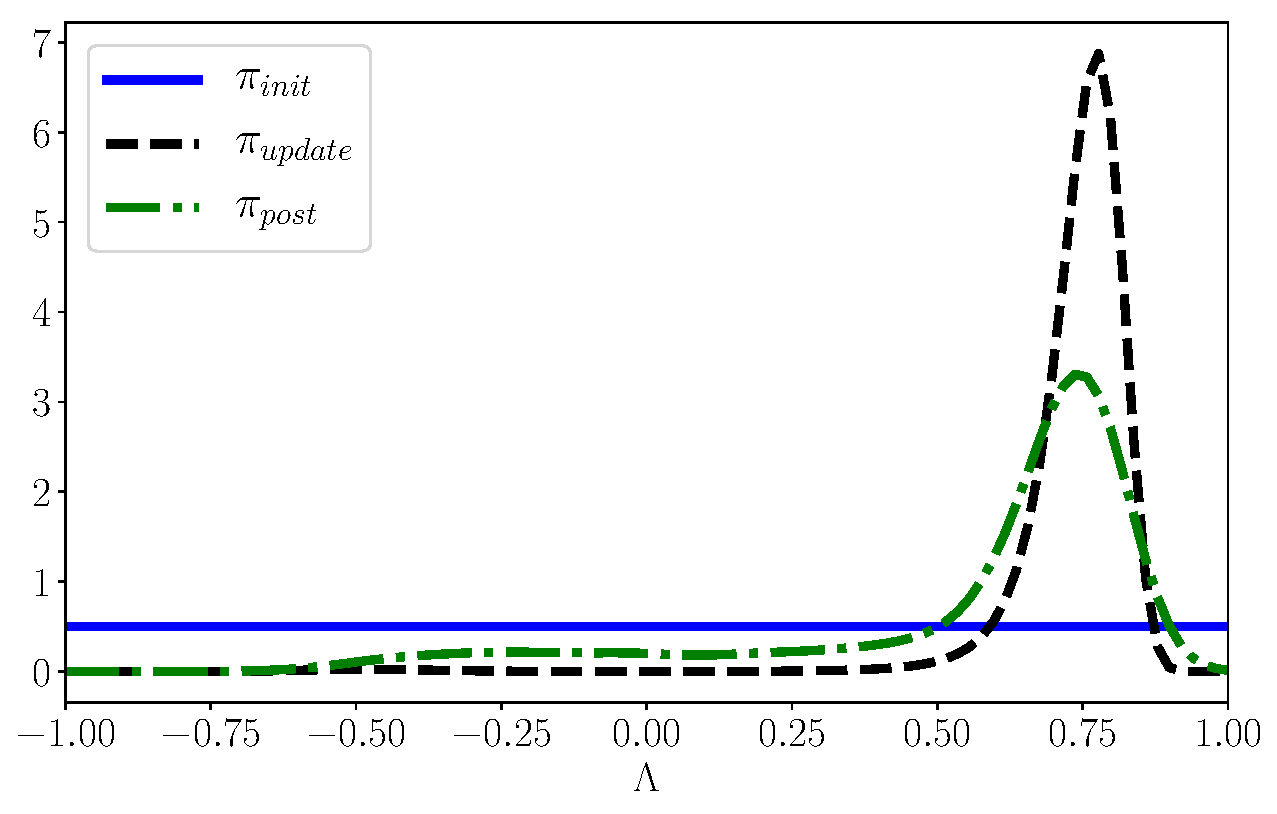
\includegraphics[width=0.49\linewidth]{figures/cbayes_comp_sbayes_50000_paramdens_nonlinear-standalone.pdf}
   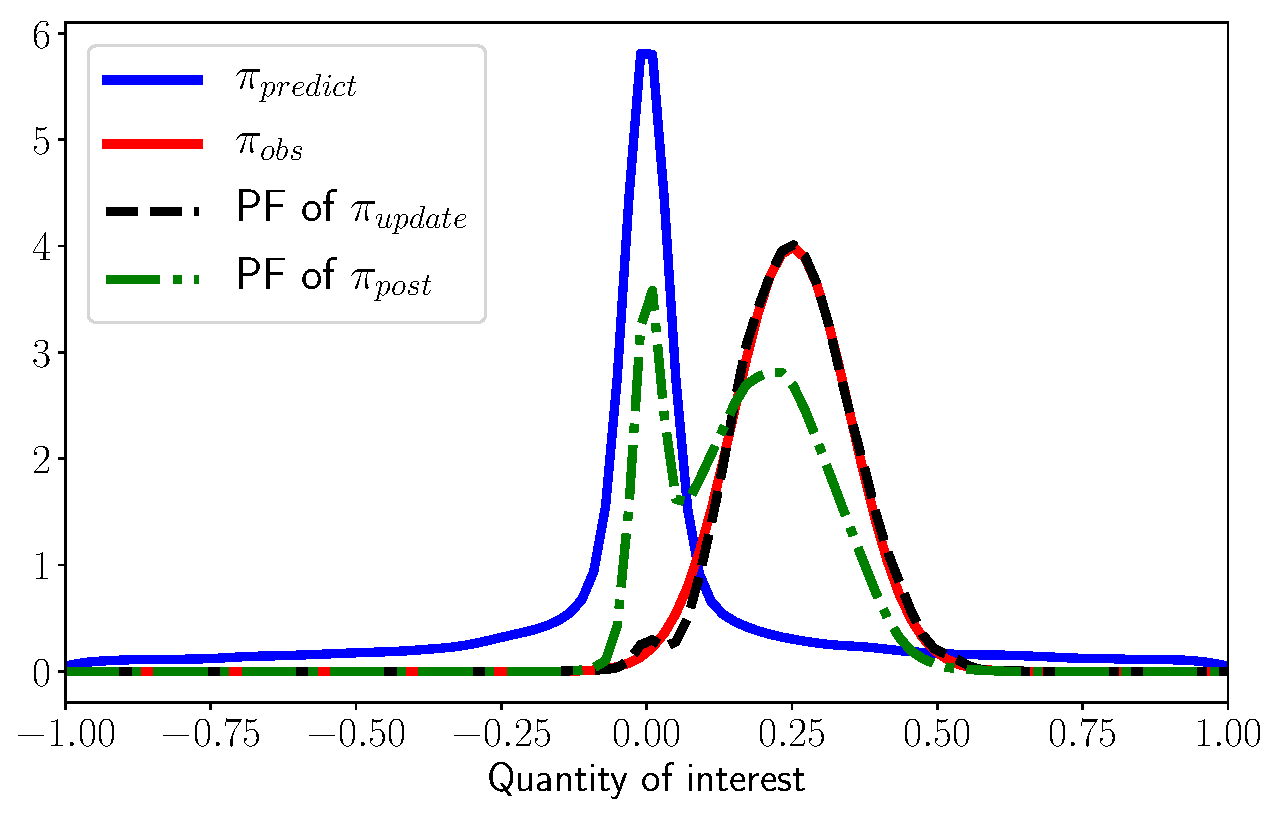
\includegraphics[width=0.49\linewidth]{figures/cbayes_comp_sbayes_50000_outdens_nonlinear-standalone.pdf}
 \caption{(Left) The initial/prior PDF $\initial$ (blue solid curve), updated PDF $\updated$ (black dashed curve), and posterior PDF $\pi_\text{post}$ (green dashed-dotted curve) on $\Lambda$.
 (Right) The push-forward (PF) of the initial/prior PDF $\predicted$ (blue solid curve), observed/likelihood PDF (red solid curve), PF of the updated PDF $\updated$ (black dashed curve), and the PF of the posterior PDF $\pi_\text{post}$ (green dashed-dotted curve) for the QoI.}
 \label{fig:bayes-comparison}
\end{figure}

The takeaway to the above discussion and example is that each density is solving a {\em different} inverse problem.
The posterior density is intended to provide point estimates of a true parameter value whereas the updated density is intended to quantitatively characterize natural variations in parameter values.

Suppose we reformulated this example slightly to make the role of data more central.
Specifically, suppose $Q(\paramref)=0.25$ and noisy measurement data are drawn from a $N(0.25,0.1^2)$, i.e., we assume that $d=Q(\paramref)+\xi$ where $\xi\sim N(0,0.1^2)$.
For the SIP, we could use the sample mean and variance of this data to estimate the ``exact'' observed $N(0.25,0.1^2)$ distribution whereas the data-likelihood would involve a product of normal densities.
In this case, the objective is to use the posterior or updated density to produce an estimate of $\paramref$.
In the next section, we motivate the use of the maximal updated density point as a means of providing a useful point estimate to parameters.


%A critical component in the Bayesian framework is the prior density, which encodes any knowledge or assumptions about them input (parameter) space that we may wish to impose before any data are observed.
%In some cases, the prior and initial densities may be both specified and interpreted identically.
%However, in the Bayesian framework, the impact of the prior on the posterior density is perhaps best understood as a regularization term that makes the inverse problem well--posed by penalizing parameters uninformed by the data.
%Ideally, the prior should not interfere with well--informed parameters, i.e., parameters informed by the data.
%{Unfortunately, well--informed parameters are not known a priori and none of the existing prior elicitation approaches avoid polluting data--informed directions in the parameter space.}



%%%%%


\begin{ex}
Consider
\begin{equation}
u(\param) = \param^p
\end{equation}
for $p$ chosen as either 1 or 5.
For both approaches, the prior and initial density is given by a uniform distribution on $U[-1,1]$.
In the Data-Consistent Inversion framework, $\observed \sim \mathcal{N}(0.25,0.1^2)$.
In the statistical Bayesian framework, we take $\q=0.25$ as the datum and assume an additive error noise model with distribution $\mathcal{N}(0,0.1^2)$ so that the likelihood, $L_\dspace(\q | \param)$, matches the observed density as a function of $\param$.

When $p=1$, we have $\predicted = \frac{1}{2} = C$.
Since $\observed\Q = L_\dspace(\q|\param)$ and $\predicted$ agrees with the normalizing constant $C$, the posterior and update agree on $\pspace$ (we show the push-forwards in the right plot of Figure~\ref{fig:comparison}).
When $p=5$, the non-linearity of the model causes the push-forward of $\initial$ to be non-constant, so the two approaches now yield differing solutions, as seen in the left plot of Figure~\ref{fig:comparison}).
The push-forward of the posterior associated with the statistical Bayesian framework is influenced by the push-forward of the prior in a way that the push-forward of the updated density avoids.

\begin{figure}
\begin{minipage}{.45\textwidth}
		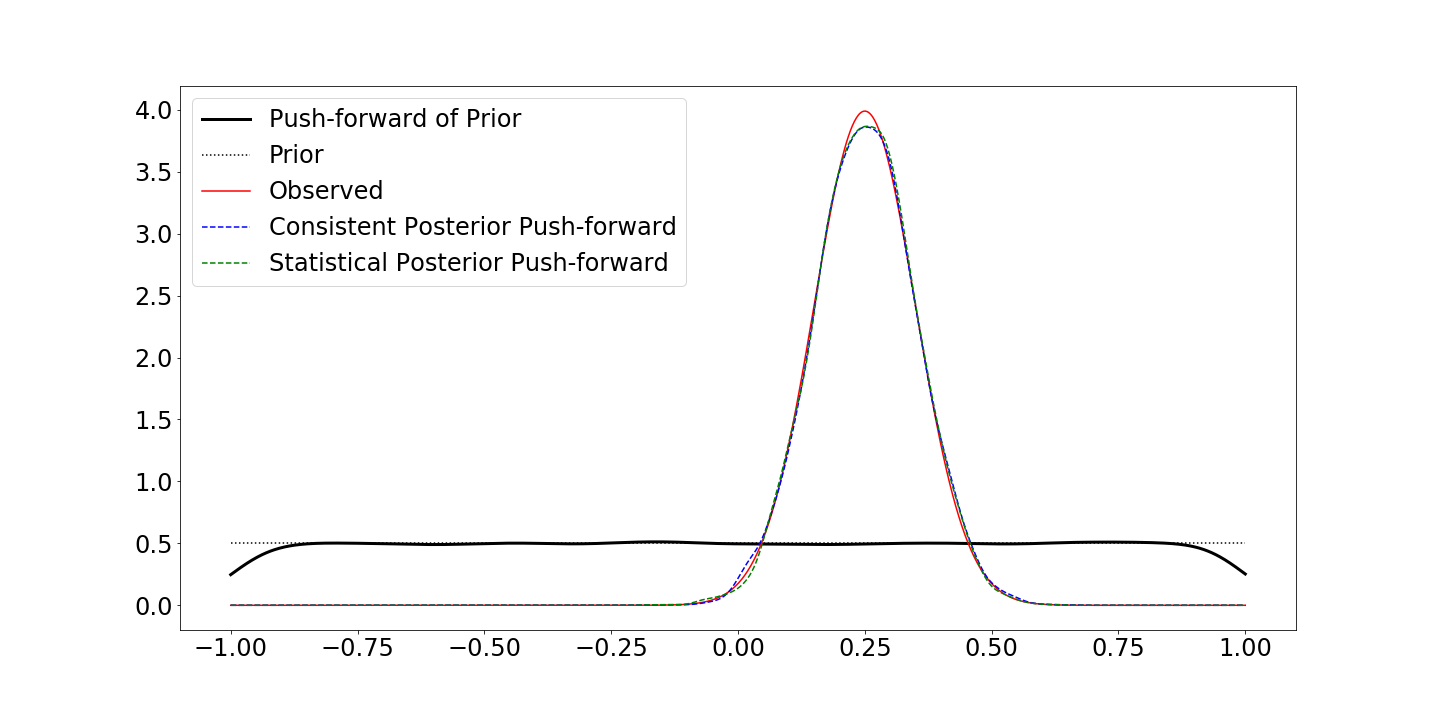
\includegraphics[width=\linewidth]{./images/comparison1}
\end{minipage}
\begin{minipage}{.45\textwidth}
		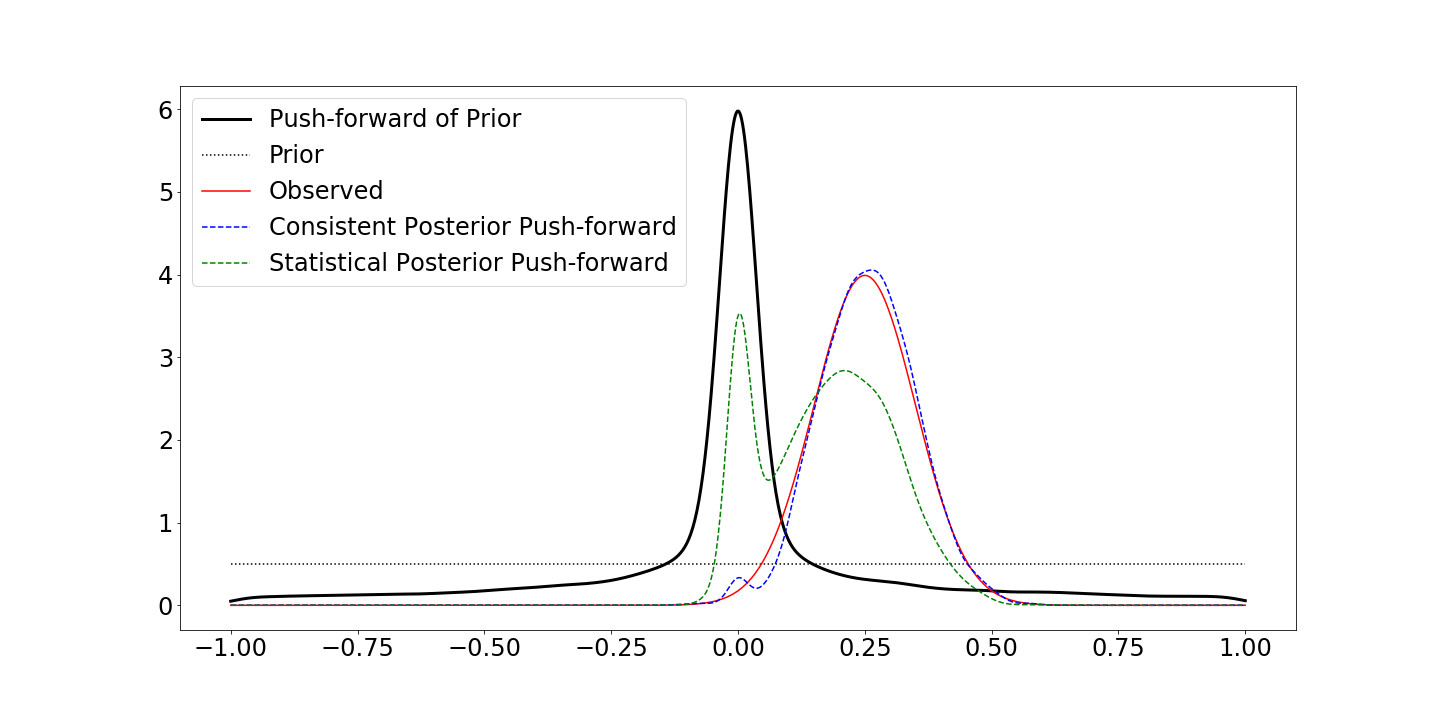
\includegraphics[width=\linewidth]{./images/comparison5}
\end{minipage}
\caption{
In each plot, the black dotted line represents the prior (initial), while the solid line represents the push-forward.
The push-forwards of the posterior (updated) densities are shown as a green (blue) dotted line.
The likelihood (observed density) is shown as a solid red line.
(Left): $p = 1$, the push-forwards of the solutions are identical because a linear map results in a constant push-forward of a uniform prior.
(Right): $p = 5$, the non-linearity of the map causes the solutions to be different and thus the push-forwards to also be different.
}
\label{fig:comparison}
\end{figure}

% [TK - removed paragraph] We can see in Figure~\ref{fig:comparison} that the two approaches pose different questions and thus yield different results.
% The Data-Consistent Inversion framework seeks to recreate the observed density, which it does for both $p=1$ and $p=5$, but the Bayesian approach is a combination of both the observed and the push-forward of the prior.
[TK - a lot of this discussion is well-covered in the intro to the mud paper... let's move it here??]
In summary, it is not the goal of Bayesian inference to construct a pullback distribution.
Bayesian inverse problems are fundamentally posed as parameter-identification, not distribution estimation.
However, one could assume that a posterior on $\pspace$ can be expressed as a Gaussian distribution, and solve for the most likely mean and standard deviation that characterizes it [TK - cite more] \cite{Smith}.
This defines what is commonly referred to a as a Hierarchical Bayesian Inverse Problem.
More complex densities can be approximated by mixture models.
For example, one can assume that the posterior can be given by a linear combination of four Gaussian distributions, and solve for eight parameter values (four standard deviations and means).
However, the operative word here is \emph{assume}; in order to capture a density using a Bayesian framework, one needs to impose some sort of explicit structure on the posterior.
No such compromise is required in the Data-Consistent Inversion framework.
Distributions (or measures) can be solved for directly, regardless of any nonlinear/non-parameteric structure by leveraging the measure-theoretic approach described in \cite{BE13} or \cite{BJW18}.

\end{ex}
